%%%%%%%%%%%%%%%%%%%%%%%%%%%%%%%%%%%%%%%%%%%%%%%%%%%%%%%%%%%%%%%%%%%%%%%%%%%%%%%
%                                                                             %
% Anwendungsbeispiel für das Beamer-Template TU Chemnitz                      %
% (c) Mario Haustein (mario.haustein@hrz.tu-chemnitz.de), 2013-2019           %
%                                                                             %
%%%%%%%%%%%%%%%%%%%%%%%%%%%%%%%%%%%%%%%%%%%%%%%%%%%%%%%%%%%%%%%%%%%%%%%%%%%%%%%

\documentclass[10pt]{beamer}

\usepackage{ifxetex}
\usepackage{ifluatex}
\ifxetex
\usepackage[babelshorthands]{polyglossia}
\setmainlanguage{german}
\else\ifluatex
\usepackage[babelshorthands]{polyglossia}
\setmainlanguage{german}
\else
\usepackage[T1]{fontenc}
\usepackage[utf8]{inputenc}
\usepackage[ngerman]{babel}
\usepackage{listingsutf8}
\fi\fi
\usepackage{url}
\usepackage{tikz}
\usepackage{amsmath}
\usepackage{exscale}
\usepackage{listings}
\usepackage{textcomp}
\usepackage{chemfig}
\usepackage{metalogo}
\usepackage{tabularx}
\usepackage{eurosym}


% Trennstellen für URLs
\def\UrlBreaks{\do\:\do\.\do\@\do\\\do\/\do\!\do\_\do\|\do\;\do\>\do\]%
 \do\)\do\,\do\?\do\'\do+\do\=\do\#}
\def\UrlBigBreaks{}

% Voreinstellungen für Quellcodelistings
\lstset{basicstyle=\ttfamily,keywordstyle=\sffamily\bfseries,breaklines,tabsize=2}
\ifxetex\else\ifluatex\else\lstset{inputencoding=utf8/latin1}\fi\fi
\lstdefinestyle{block}{basicstyle=\ttfamily,keywordstyle=\sffamily\bfseries,breakindent=10pt}
\lstdefinestyle{numberedblock}{basicstyle=\ttfamily,keywordstyle=\sffamily\bfseries,numbers=left,numberstyle=\scriptsize,xleftmargin=20pt,frame=leftline,breakindent=10pt}

% TUC-Templates laden.
\usetheme[fakcolor=ma]{tuc2019}
\newcommand{\function}[3]{#1: #2 \longrightarrow #3}
\newcommand{\stern}{\left( \ast \right)}
\newcommand{\integral}[4]{\int_{#1}^{#2} #3 \mathrm{d}#4}
\newcommand{\R}{\mathbb{R}}
\newcommand{\N}{\mathbb{N}}
\newcommand{\NN}{2\mathbb{N}}
\newcommand{\produkt}[2]{\prod_{#1}^{#2}}
\newcommand{\Z}{\mathbb{Z}}
\newcommand{\C}{\mathbb{C}}
\newcommand{\sinc}[1]{\mathrm{sinc}\left( #1 \right)}
\newcommand{\bs}{\bm}
\newcommand{\summe}[2]{\sum_{#1}^{#2}}
\newcommand{\mi}{\mathrm{i}}
\newcommand{\D}{\mathbb{T}}
\newcommand{\I}[2]{I_{#1}^{(#2)}}
\newcommand*\ematrix[5]{\begin{pmatrix}#1\end{pmatrix}_{#2,#4}^{\ \mathclap{#3}\hphantom{#2}#5}}
\newcommand{\vektor}[3]{\left( #1 \right)_{#2}^{#3}}
\newcommand{\norm}[1]{\left\lVert#1\right\rVert}
\newcommand{\num}[1]{\left\{1,2,\dots ,#1\right\} }
\newcommand{\order}[2]{ #1 = 1, 2, \dots , #2 }
\newcommand{\abs}[1]{\left| #1 \right| }
\DeclareMathOperator*{\argmin}{arg\,min}
\DeclareMathOperator*{\argmax}{arg\,max}
\DeclareRobustCommand{\rchi}{{\mathpalette\irchi\relax}}
\newcommand{\irchi}[2]{\raisebox{\depth}{$#1\chi$}}
\newcommand{\skalar}[2]{\left\langle #1 , #2 \right\rangle}
\newcommand{\munderbar}[1]{\underline{#1}}
\renewcommand{\bar}{\overline}
\newcommand{\LSQR}[2]{\mathrm{LSQR}(\bs{F},#1,\epsilon_{\mathrm{tol}},i_{\text{max}})~\text{mit}~\bs F = \bs{F}(N,M,\bs{X},#2)}
\newcommand{\NFFT}[2]{\mathrm{NFFT}(N,M,\bs X,#1,#2)}
\newcommand{\highl}[1]{\color{tuccolor@ma}#1\color{black}}
\mode<article>{\usepackage{beamerarticletuc2019}}


%  Metadaten
\title[Orientierungswoche Mathematik 2021]{Orientierungswoche Mathematik 2021}
\author{FSR Mathematik}
\date{04.10.2021}
\institute[]{TU Chemnitz}
\titlegraphic{
\includegraphics[height=0.2\textheight]{tuc2019/logo/tuc_green}}
\tucurl{http://www.tu-chemnitz.de/fsrmathe/}
\setbeamertemplate{navigation symbols}{}

\definecolor{presentationblue}{RGB}{0,119,187}


\begin{document}

\begingroup

\tucthreeheadlines

\frame{\frametitle{Ablauf}\tableofcontents}

\endgroup

\tuctwoheadlines

\section{Hygienekonzepte}

\begin{frame}
	\frametitle{Hygienekonzepte}
	\begin{itemize}
		\item Hat jemand das Hygienekonzept der TU Chemnitz und das Hygienekonzept der Orientierungswoche in Papierform nicht erhalten?
		\item Vorlesen der Hygienekonzepte.
		\item Wer an Veranstaltungen in Präsenz teilnehmen möchte, verpflichtet sich zur Einhaltung beider Hygienekonzepte!
		\item Habt Ihr noch Fragen?
	\end{itemize}
\end{frame}


\section{Begrüßung}

\begin{frame}
	\begin{center}
		\Huge{\highl{Begrüßung durch den Dekan Prof.~Dr.~Oliver Ernst}}
	\end{center}
\end{frame}

\begin{frame}
	\frametitle{Umfragen}

	\begin{itemize}
		\item In welchen Studiengang seid Ihr eingeschrieben?
		\item Woher kommt Ihr?
		\item Wohnt Ihr in der Nähe der Universität (mit einem Internetzugang)?
	\end{itemize}
\end{frame}

\begin{frame}
	\frametitle{Wochenplan}

	\begin{center}

		\begin{tabular}{p{2cm}|p{1.9cm}|p{2.3cm}|p{1.9cm}|p{2cm}}

			\textbf{Montag}\newline 04.10.2021
			&\textbf{Dienstag}\newline 05.10.2021
			&\textbf{Mittwoch}\newline 06.10.2021
			&\textbf{Donnerstag}\newline 07.10.2021
			&\textbf{Freitag}\newline 08.10.2021\\\hline

			
			&\textit{09:45-14:00} \newline \textbf{Campustour}
			&\textit{10:00-11:00} \newline \textbf{Mentoring}
			&\textit{09:45-14:00} \newline \textbf{Stadttour}
			&\textit{9:00-11:00} \newline \textbf{Fachstudien- beratung} \\\hline

			\textit{13:00-15:00} \newline \textbf{Begrüßung}
			&
			&\textit{11:00-12:00} \newline \textbf{Einführungs- kurs}
			&
			&\textit{11:00-12:00} \newline \textbf{Einführungs- kurs} \\\hline

			\textit{16:00-17:00} \newline \textbf{Einführungs- kurs}
			&
			&\textit{14:30-17:00} \newline \textcolor{red}{URZ \& MRZ Stundenplan}
			&
			&\\\hline

			\textit{ab 19:00} \newline Erstis meet FSR
			&
			&\textit{ab 19:00} \newline Digitaler Cocktailabend
			&
			&
		\end{tabular}
	\end{center}

	Alle Infos: \highl{\textit{\href{https://www.stura.tu-chemnitz.de/fsrmathe/events/o-phase}{https://www.stura.tu-chemnitz.de/fsrmathe/events/o-phase}}}
\end{frame}

\begin{frame}

	\frametitle{Wichtige Hinweise}

	\begin{itemize}
		\item Bitte denkt an \textbf{Euren Impf- oder Genesenennachweis oder Euren Nachweis für einen tagesaktuellen negativen Coronatest} und zeigt diesen vor jeder Veranstaltung in Präsenz der zuständigen Person des Fachschaftsrates!
		\item Bitte haltet \textbf{immer} die \textbf{Hygienekonzepte} ein!
		\item Bitte bringt einen Stift mit!
		\item Bitte bringt Euch zur Campus- und Stadttour selbst \textbf{Getränke und Verpflegung} mit! Und denkt an warme Klamotten!
		\item \highl{Die O-Phase dient vor allem dem Networking -- nutzt diese Chance!}
	\end{itemize}
\end{frame}


\section{Fachschaftsrat Mathematik}
\frame{\tableofcontents[currentsection]}

\begin{frame}
	\frametitle{Wer sind wir eigentich?}

	\begin{block}{\vphantom{X}\smash{Fachschaft}}
		Als Fachschaft bezeichnet man den Zusammenschluss aller Studierenden einer Fakultät bzw. eines Instituts.
	\end{block}

	\begin{itemize}
		\item Der Fachschaftsrat ist die gewählte Vertretung dieser Studierenden mit bis zu 15 Mitgliedern.
		\item Wahlen finden jedes Jahr zum Beginn des Wintersemesters statt.
		\item Jedes Mitglied der Fachschaft kann sich aufstellen lassen und damit auch \textbf{Ihr}!
		\item \highl{Ihr dürft und solltet wählen gehen!}
	\end{itemize}
\end{frame}

\begin{frame}
	\frametitle{Wer sind wir eigentlich?}

	Im Moment hat der FSR 7 gewählte Mitglieder:

	\begin{itemize}
		\item Lina Lehnert, \textit{Master Mathematik}
		\item Svenja Schürer, \textit{Master Mathematik}
		\item Felix Naake, \textit{Master Mathematik}
		\item Tom-Christian Riemer, \textit{Master Mathematik}
		\item Jeremias Piljug, \textit{Master Mathematik}
		\item Lina Bohse, \textit{Bachelor Finanzmathematik}
		\item Lisa Wilms, \textit{Bachelor MINT}
	\end{itemize}

	Und weiteren beratenden Mitgliedern!
\end{frame}

\begin{frame}
	\frametitle{Was sind unsere Aufgaben?}

	\begin{itemize}
		\item Wir verfügen über etwa 1000\euro{} an Fachschaftsmitteln jedes Semester.
		\item Diese nutzen wir für diverse Veranstaltungen: O-Phase, Grillen, Weihnachtsfeier, Sporttag, \ldots
		\item Der FSR führt außerdem Lehrevaluationen durch und vertritt Eure Interessen gegenüber der Fakultät (Universität).
		\item Besondere, regelmäßige Angebote (außerhalb von Corona):
			\begin{itemize}
				\item Spieleabend: jeden 2. Mittwoch ab 19 Uhr im Fakultätsgebäude.
				\item DFM: Fußball mit Turnier der Mathematikfachschaften jeden Sommer .
				\item KoMa: Konferenz der deutschsprachigen Mathematikfachschaften.
			\end{itemize}
	\end{itemize}
\end{frame}


\section{Wie geht das Studieren?}
\frame{\tableofcontents[currentsection]}


\begin{frame}
	\frametitle{Studium - Wie funktioniert das eigentlich?}

	\begin{block}{\vphantom{X}\smash{Ordnungen}}
		Das Studium ist durch 2 Ordnungen geregelt: Die \textbf{Studienordnung} und die \textbf{Prüfungsordnung}. Diese Dokumente sind verbindlich und Ihr könnt Euch auf diese berufen.
	\end{block}

	\begin{itemize}
		\item Früher oder später muss jeder diese Dokumente anschauen!
		\item Wo finde ich meine Ordnungen? $\Rightarrow$ Website$\rightarrow$Fakultäten (Mathematik)$\rightarrow$Studium$\rightarrow$Studiengänge$\rightarrow$\textit{Euer Studiengang}$\rightarrow$Informationen.
	\end{itemize}

	\vspace*{1.0cm}

	\highl{\textit{\href{https://www.tu-chemnitz.de/mathematik/studium/content_studiengaenge.de.php}{https://www.tu-chemnitz.de/mathematik/studium/content\_studiengaenge.de.php}}}
\end{frame}

\begin{frame}
	\frametitle{Was steht in den Ordnungen?}

	\begin{itemize}
		\item Studienordnung:
			\begin{itemize}
				\item Welche Veranstaltungen muss ich besuchen?
				\item Welche Veranstaltungen soll ich in Semester X besuchen? $\Rightarrow$ Freie Wahl, aber Orientierung an Studienablaufplan ist gut. $\Rightarrow$ In der Praxis: Vorlesungsverzeichnis: \highl{\textit{\href{https://www.tu-chemnitz.de/verwaltung/vlvz/plan/mathe/}{https://www.tu-chemnitz.de/verwaltung/vlvz/plan/mathe/}}}
				\item Mittwoch ab 14:30: \textbf{Stundenplanung}!
				\item Modulbeschreibungen: Lehrinhalte, Prüfungsvorleistungen, Prüfungsart, Prüfungsdauer, \ldots
			\end{itemize}
		\item Prüfungsordnung:
			\begin{itemize}
				\item Fristen, Zulassungsverfahren, Arten der Prüfungsleistungen, Rücktritt, Anrechnung von Prüfungsleistungen, \ldots 
			\end{itemize}
	\end{itemize}
\end{frame}

\begin{frame}
	\frametitle{Welche Studiengänge gibt es?}

	\begin{itemize}
		\item Bachelor of Science (B.Sc.)
			\begin{itemize}
				\item Mathematik
				\item Finanz- und Wirtschafts­mathematik
				\item MINT
			\end{itemize}
		\item Master of Science (M.Sc.)
			\begin{itemize}
				\item Mathematik
				\item Data Science
				\item Finance
			\end{itemize}
		\item Diplom Mathematik (Dipl.)
		\item Internationaler Master- und Promotions­studiengang
	\end{itemize}
\end{frame}

\begin{frame}
	\frametitle{Was ist (m)ein Nebenfach?}

	\highl{Wichtig für Mathematik B.Sc.!}

	\begin{itemize}
		\item Mathematik wird generell nie allein studiert, immer mit einer Art von Nebenfach. Dies soll Euch für den Arbeitsmarkt „attraktiver“ machen!
		\item Es gibt Chemie, Physik, Informatik, Maschinenbau, Elektrotechnik, Wirtschaftswissenschaften, Sensorik und Kognition sowie Psychologie als Nebenfach!
		\item Es müssen 24 (max. 26) LP von 180 LP aus Modulen \textbf{eines} Nebenfachs (und Ergänzungsmodulen) besucht werden. Die Wahl der Module innerhalb des Nebenfachs ist frei!
		\item Man legt sein Nebenfach indirekt über die Anmeldung der entsprechenden Prüfungen fest.
		\item Wechsel des Nebenfachs ist jederzeit möglich $\Rightarrow$ Ausprobieren verschiedener Nebenfächer kann sehr hilfreich sein!
		\item Studienberater: Prof. Dr. Vladimir Shikhman
	\end{itemize}
\end{frame}

\begin{frame}
	\frametitle{Was ist (m)ein Nebenfach?}

	\highl{Wichtig für Finanz- und Wirtschafts­mathematik B.Sc.!}

	\begin{itemize}
		\item Ihr habt sozusagen ein „festes“ Nebenfach!
		\item Es müssen 24 LP aus Modulen der Wirtschaftswissenschaften besucht werden.
		\item Zusätzlich müssen 15 (max. 18) LP aus Vertiefungsmodulen der Wirtschaftswissenschaften (und Ergänzungsmodulen) besucht werden. Die Wahl der Vertiefungsmodule ist frei!
		\item Studienberater: Prof. Dr. Alois Pichler, Prof. Dr. Vladimir Shikhman
	\end{itemize}
\end{frame}

\begin{frame}
	\frametitle{Was ist (m)eine Spezialisierungsrichtung?}

	\highl{Wichtig für MINT B.Sc.!}

	\begin{itemize}
		\item Der Studiengang setzt sich zusammen aus Orientierungsstudium, Spezialisierungsstudium und Forschungsstudium. 
		\item Im Orientierungsstudium müssen 64 LP aus Modulen der Mathematik, der Informatik und der Physik besucht werden.
		\item Ihr entscheidet Euch für \textbf{eine} dieser Disziplinen als Eure Spezialisierungsrichtung in welcher Ihr 96 LP erbringen müsst.
		\item Man legt seine Spezialisierungsrichtung indirekt über die Anmeldung der entsprechenden Prüfungen fest.
		\item Wechsel möglich, aber nicht einfach!
		\item Das Forschungsstudium setzt sich aus einem Modellierungsseminar und der Bachelor-Arbeit zusammen.
		\item Studienberater: Prof. Dr. Peter Stollmann
	\end{itemize}
\end{frame}

\begin{frame}
	\frametitle{Was ist (m)eine Studienrichtungen?}

	\highl{Wichtig für Diplom Mathematik!}

	\begin{itemize}
		\item Im Diplomstudiengang gibt es die Studienrichtungen Mathematik (MMM), Wirtschaftsmathematik (WMM), Finanzmathematik (FMM), Mathematik mit vertiefter Informatik (IMM), Technomathematik (TMM).
		\item Studienrichtung Mathematik ist mit einem der Nebenfächer Chemie, Elektrotechnik, Maschinenbau, Medizintechnik, Physik, Wirtschaftswissenschaften oder Informatik zu wählen.
		\item Studienrichtungen unterscheiden sich im Anteil zwischen Nebenfach und Mathematik.
		\item Man legt seine Studienrichtung indirekt über die Anmeldung der entsprechenden Prüfungen fest.
		\item Wechsel der Studienrichtung ist jederzeit möglich!
		\item Studienberater: Prof. Dr. Vladimir Shikhman
	\end{itemize}
\end{frame}

\begin{frame}
	\frametitle{Prüfungen\dots}

	\begin{itemize}
		\item Prüfungen sind (wie das gesamte Studium) geregelt. Die Prüfungsanmeldung erfolgt während der Vorlesungszeit (Wintersemester: Dezember).
		\item Wie melde ich mich an? $\Rightarrow$ über den SB-Service \highl{\textit{\href{https://www.tu-chemnitz.de/studentenservice/zpa/pruefungsanmeldung}{https://www.tu-chemnitz.de/studentenservice/zpa/pruefungsanmeldung}}} \\
		\highl{NICHT IM STUDIUM GENERALE ANMELDEN!!!}
		\item Prüfungsanmeldungen sind verbindlich $\Rightarrow$ Wer nicht auftaucht, fällt durch. 
		\item Rücktritt von der Prüfung bis 1 Woche vor dem Klausurtermin. Bei mündlichen Prüfungen bis eine Woche vor Semesterende.\\
		\highl{Teilt das trotzdem dem Prüfer (üblicherweise Prof.) mit!}
		\item Bei Krankheit: Entweder direkt zum Arzt und den Krankenschein ins ZPA bringen oder zumindest das ZPA benachrichtigen.
		\item Wann finden Prüfungen statt? In der „zentralen Prüfungsperiode“ nach dem Prüfungsplan $\Rightarrow$ \highl{\textit{\href{https://www.tu-chemnitz.de/studentenservice/zpa/pruefungsplaene.php}{https://www.tu-chemnitz.de/studentenservice/zpa/pruefungsplaene.php}}}
	\end{itemize}
\end{frame}

\begin{frame}
	\frametitle{Lehrveranstaltungen: Vorlesung, Übung, Seminar, \ldots}

	\begin{itemize}
		\item Eine Lehrveranstaltung ($\approx$ Unterricht zum Modul) umfasst mehrere Einheiten pro Woche, die Vorlesungen, Übungen, Seminare oder Praktika sein können. 
		\item Es gibt verschiedene Standardformen: 4+4, 4+2, 2+2, 3+1, \ldots
		\item Die Prüfung einer Lehrveranstaltung kann Inhalte aus allen Teilen umfassen.
		\item Stil von Mathematikveranstaltungen: überwiegend mit Kreide auf Tafel.
		\item Tipp: gutes Schreibwerkzeug besorgen!
		\item teaser: Einführungskurse.
	\end{itemize}
\end{frame}


\section{Ansprechpartner und Gremien}
\frame{\tableofcontents[currentsection]}

\begin{frame}
	\frametitle{Fragen -- An wen kann ich mich wenden?}

	Ihr seid im Gegensatz zur Schule ab jetzt komplett für Euch alleine verantwortlich! Wenn Ihr Fragen oder Probleme habt, dann müsst Ihr selbst aktiv werden!

	\begin{block}{\vphantom{X}\smash{FSR Mathe}}
		Der FSR ist eine gute erste Anlaufstelle \textbf{für alle Probleme} und wenn Ihr nicht sicher seid, an wen Ihr Euch sonst wenden sollt.
	\end{block}

	\begin{itemize}
		\item FSR-Büro: Reichenhainer Str. 41/001 [siehe Campustour]
		\item FSR-Mail: \highl{\textit{\href{mailto:fachschaft@mathematik.tu-chemnitz.de}{fachschaft@mathematik.tu-chemnitz.de}}}
		\item FSR-Telefon: 0371/531 - 16200
		\item Die Mail-Adressen der einzelnen Mitglieder findet Ihr auf unserer Internetseite \highl{\textit{\href{https://www.stura.tu-chemnitz.de/fsrmathe/mitglieder}{www.stura.tu-chemnitz.de/fsrmathe/mitglieder}}}.
	\end{itemize}
\end{frame}

\begin{frame}
	\frametitle{Fragen -- An wen kann ich mich wenden?}

	Ihr findet alle Gremien der Fakultät und ihre Mitglieder online unter 

	\vspace*{1.0cm}

	\begin{center}
		\highl{\textit{\href{https://www.tu-chemnitz.de/mathematik/fakultaet/gremien.de.php}{https://www.tu-chemnitz.de/mathematik/fakultaet/gremien.de.php}}}
	\end{center}
\end{frame}

\begin{frame}
	\frametitle{Fragen -- An wen kann ich mich wenden?}

	\begin{block}{\vphantom{X}\smash{Fakultätsrat}}
		Der Fakultätsrat ist das wichtigste Gremium der Fakultät.
	\end{block}

	\begin{itemize}
		\item Die zwei studentischen Mitglieder werden jährlich bei den Universitätswahlen gewählt.
	\end{itemize} 

	\vspace*{1.0cm}

	Aktuelle Mitglieder:

	\begin{itemize}
		\item Tom-Christian Riemer: \highl{\textit{\href{mailto:tom.riemer@math.tu-chemnitz.de}{tom.riemer@math.tu-chemnitz.de}}}
		\item Lina Bohse: \highl{\textit{\href{mailto:lina.bohse@s2018.tu-chemnitz.de}{lina.bohse@s2018.tu-chemnitz.de}}}
	\end{itemize}
\end{frame}

\begin{frame}
	\frametitle{Fragen -- An wen kann ich mich wenden?}

	\begin{block}{\vphantom{X}\smash{Studienkommission}}
		Die Studienkommission führt die Lehrevaluationen mit dem FSR zusammen durch und bearbeitet die Studiendokumente.
	\end{block}

	\begin{itemize}
		\item Es gibt für jeden Studiengang eine Studienkommission.
		\item Die studentischen Mitglieder werden durch den Fakultätsrat bestimmt.
	\end{itemize}
\end{frame}

\begin{frame}
	\frametitle{Fragen -- An wen kann ich mich wenden?}

	\begin{block}{\vphantom{X}\smash{Prüfungsausschuss}}
		Der Prüfungsausschuss hat weitreichende Aufgaben um das Prüfungsgeschehen und entscheidet über Anträge.
	\end{block}

	\begin{itemize}
		\item Die studentischen Mitglieder werden durch den Fakultätsrat bestimmt.
	\end{itemize}

	\vspace*{0.5cm}

	Aktuelle Mitglieder:

	\begin{itemize}
		\item Josie König (Mathematik Bachelor \& Diplom, Fi- \& WiMa Bachelor): \highl{\textit{\href{mailto:josie.koenig@s2016.tu-chemnitz.de}{josie.koenig@s2016.tu-chemnitz.de}}}
		\item Tom-Christian Riemer (Mathematik Bachelor \& Diplom): \highl{\textit{\href{mailto:tom.riemer@math.tu-chemnitz.de}{tom.riemer@math.tu-chemnitz.de}}}
		\item Lisa Wilms (MINT): \highl{\textit{\href{mailto:lisa.wilms@s2018.tu-chemnitz.de}{lisa.wilms@s2018.tu-chemnitz.de}}}
	\end{itemize}
\end{frame}

\begin{frame}
	\frametitle{Fragen -- An wen kann ich mich wenden?}

	\begin{block}{\vphantom{X}\smash{Strukturkommission}}
		Die Strukturkommission gibt Empfehlungen zur Besetzung von Haushaltsstellen.
	\end{block}

	\begin{itemize}
		\item Das studentische Mitglied wird durch den Fakultätsrat bestimmt.
	\end{itemize}

	\vspace*{1.0cm}

	Aktuelles Mitglied:

	\begin{itemize}
		\item Tom-Christian Riemer: \highl{\textit{\href{mailto:tom.riemer@math.tu-chemnitz.de}{tom.riemer@math.tu-chemnitz.de}}}
	\end{itemize}
\end{frame}

\begin{frame}
	\frametitle{Fragen -- An wen kann ich mich wenden?}

	\begin{block}{\vphantom{X}\smash{Stipendienkommission}}
		Die Stipendienkommission befasst sich mit der Vergabe des Deutschlandstipendiums.
	\end{block}

	\begin{itemize}
		\item Das studentische Mitglied wird durch den Fakultätsrat bestimmt.
	\end{itemize}

	\vspace*{1.0cm}

	Aktuelles Mitglied:
	\begin{itemize}
		\item Josie König: \highl{\textit{\href{mailto:josie.koenig@s2016.tu-chemnitz.de}{josie.koenig@s2016.tu-chemnitz.de}}}
	\end{itemize}
\end{frame}

\begin{frame}
	\frametitle{Fragen -- An wen kann ich mich wenden?}

	\begin{block}{\vphantom{X}\smash{Haushaltskommission}}
		Die Haushaltskommission befasst sich mit dem Haushalt der Fakultät und dessen Verteilung.
	\end{block}

	\begin{itemize}
		\item Das studentische Mitglied wird durch den Fakultätsrat bestimmt.
	\end{itemize}

	\vspace*{1.0cm}

	Aktuelles Mitglied:

	\begin{itemize}
		\item Kira Reker: \highl{\textit{\href{mailto:kira.reker@s2014.tu-chemnitz.de}{kira.reker@s2014.tu-chemnitz.de}}}
	\end{itemize}
\end{frame}

\begin{frame}
	\frametitle{Außerhalb der Fakultät -- Was gibt es noch?}
	
	\begin{block}{\vphantom{X}\smash{StuRa}}
		Der Student\_innenenrat (StuRa) ist die Vertretung aller Studierenden in der verfassten Studierendenschaft und kümmert sich z.B. um das Semesterticket.
	\end{block}

	\begin{itemize}
		\item Jede Fachschaft kann eine gewisse Zahl an Mitgliedern stellen, diese werden durch den FSR gewählt
	\end{itemize}

	\vspace*{1.0cm}

	Aktuelles Mitglied:

	\begin{itemize}
		\item leider niemand :(
	\end{itemize}
\end{frame}

\begin{frame}
	\frametitle{Außerhalb der Fakultät -- Was gibt es noch?}

	\begin{block}{\vphantom{X}\smash{Senat}}
		Der Senat ist verantwortlich für Themen, welche die gesamte Universität betreffen. Seine Zustimmung ist für viele Entscheidungen erforderlich.
	\end{block}

	\begin{itemize}
		\item Die studentischen Mitglieder werden jedes Jahr bei den Universitätswahlen gewählt.
	\end{itemize}
\end{frame}


\section{Sonstiges}
\frame{\tableofcontents[currentsection]}

\subsection*{Ehrenamtliches Engagement}

\begin{frame}
	\frametitle{Die Initiativen der TU Chemnitz}

	\vspace*{2.1cm}

	\begin{picture}(0,0)
		\put(20,-100){
\includegraphics[clip=true,trim = 10mm 55mm 10mm 5mm, width=110mm]{Initiativen.pdf}} % lo
		\put(160,-110){
\includegraphics[clip=true,trim = 5mm 250mm 155mm 5mm]{visitenkarte.pdf}} % ru
	\end{picture} \\

	\vspace*{3.8cm}

	Mehr Infos gibt es unter: \highl{\textit{\href{https://www.tu-chemnitz.de/tu/studentisches-engagement/initiativen.html}{www.tu-chemnitz.de/tu/studentisches-engagement/initiativen.html}}}.
\end{frame}

\subsection*{ }

\begin{frame}
	\frametitle{Was ist für Euch noch interessant?}

	\begin{block}{\vphantom{X}\smash{URZ}}
		Das Universitätsrechenzentrum ist verantwortlich für die digitale Infrastruktur der Universität, darunter auch Eure E-Mails.
	\end{block}

	\begin{itemize}
		\item Ihr könnt online unter \highl{\textit{\href{https://www.tu-chemnitz.de/urz/nutzerkonto.html}{https://www.tu-chemnitz.de/urz/nutzerkonto.html}}} Euren Account aktivieren!
		\item Hat das jemand noch nicht getan? Bitte nachholen!
		\item Ihr könnt dann in fast allen Computerpools mit Eurem Nutzerkennzeichen arbeiten (außer FRIZ).
		\item OPAL-Login wird dadurch ermöglicht.
		\item Einführung in die Dienste des URZ: Mittwoch online ab 14:30.
	\end{itemize}
\end{frame}

% Mit MRZ nochmal sprechen bzgl Nutzerkennzeichen. Wo abholen? Ist Repository noch gültig?
\begin{frame}
	\frametitle{Was ist für Euch noch interessant?}

	\begin{block}{\vphantom{X}\smash{MRZ}}
		Das mathematische Rechenzentrum ist verantwortlich für die digitale Infrastruktur der Fakultät für Mathematik, darunter auch die dortigen Computerpools.
	\end{block}

	\begin{itemize}
		\item Ihr müsst Euer Nutzerkennzeichen manuell über \highl{\textit{\href{https://bildungsportal.sachsen.de/opal/auth/RepositoryEntry/428277761}{bildungsportal.sachsen.de/opal/auth/RepositoryEntry/428277761}} }freischalten lassen!
		\item Bitte in das Antragsformular „einschreiben“!
		\item Damit könnt Ihr dann das Linux-Betriebssystem auf den Computern der Fakultät nutzen.
		\item Für Windows müsst Ihr Euch mit den URZ-Daten anmelden! 
		\item Einführung in die Dienste des MRZ: Mittwoch ab 14:30.
	\end{itemize}
\end{frame}

\begin{frame}
	\frametitle{Was ist für Euch noch interessant?}

	\begin{block}{\vphantom{X}\smash{Bibliothek}}
		Hier gibt es (sehr) viele Bücher!
	\end{block}

	\begin{itemize}
		\item Euer Studierendenausweis ist gleichzeitig Euer Bibliotheksausweis!
		\item Seit 2020 befindet sich die Zentralbibliothek in der alten Aktienspinnerei. Wir zeigen Euch alles bei der Stadttour.
		\item Ihr werdet wahrscheinlich nicht so viele Bücher brauchen, aber man kann dort auch ganz gut lernen!
		\item Verlängerung von Büchern geht online, auch viele E-Books: \highl{\textit{\href{https://www.tu-chemnitz.de/ub/}{www.tu-chemnitz.de/ub/}}}
		\item Benutzernummer steht auf dem Studierendenausweis. Passwort ist TTMMJJ von Eurem Geburtsdatum!
	\end{itemize}
\end{frame}

\begin{frame}
	\frametitle{Meine Buchempfehlung:}

	Tutorium Analysis 1 und Lineare Algebra 1: Mathematik von Studenten für Studenten erklärt und kommentiert, \\
	Florian Modler, Martin Kreh, \\
	Springer Verlag 

	\begin{center}
		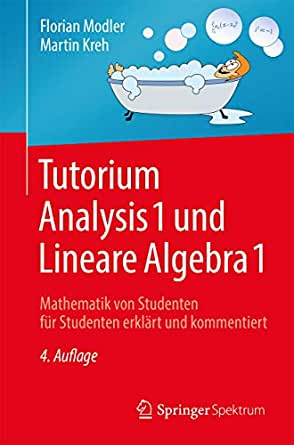
\includegraphics[width=2.5cm]{bilder/Buch.jpg}
	\end{center}

	Dieses Buch ist in der Bibliothek ausleihbar und als E-Book kostenlos über die Website der Bibliothek verfügbar!
\end{frame}

\begin{frame}
	\frametitle{Was ist für Euch noch interessant?}

	\begin{block}{\vphantom{X}\smash{Studentenwerk Chemnitz-Zwickau}}
		Das Studentenwerk kümmert sich um fast alle Anliegen der Studierenden außerhalb der Universität. Das betrifft die Finanzen, das Wohnen, die Verpflegung, Soziales \& Beratung, Kultur \& Freizeit.
	\end{block}

	Hier ist Eure Anlaufstelle für \ldots

	\begin{itemize}
		\item \ldots Inlands- und Auslands-BAföG.
		\item \ldots die Verwaltung der Studentenwohnheime.
		\item \ldots die Verwaltung der Mensa.
	\end{itemize}

	Wir werden dort bei der Campustour vorbeischauen! 
\end{frame}

\begin{frame}
	\frametitle{Was ist für Euch noch interessant?}

	\begin{block}{\vphantom{X}\smash{Mensa}}
		Hier gibt's das Essen. Wir haben zwei Mensen, davon eine hier am Campus Reichenhainer Str. und eine am Universitätsteil Straße der Nationen.
	\end{block}

	\begin{itemize}
		\item Euer Studierendenausweis ist Eure Mensakarte. Ihr könnt an zwei Automaten in der Mensa und anderswo Geld aufladen. Man kann auch in Bar bezahlen, aber Ihr müsst Euch als Studierender ausweisen, sonst zahlt Ihr mehr.
	\end{itemize}
\end{frame}

\begin{frame}
	\frametitle{Mentoring}

	\begin{block}{\vphantom{X}\smash{Mentoring}}
		Wir bieten dieses Jahr zum vierten Mal ein Programm an, bei welchem erfahrene Studierende als Mentoren von ein bis drei Erstis fungieren. Das Programm wird von der Fakultät und TU4U unterstützt. Es war in den letzten Jahren sehr erfolgreich!
	\end{block}
	
	\begin{itemize}
		\item Wir empfehlen, dass jeder die Einführungsveranstaltung besucht, welche am Mittwoch von 10:00 bis 11:00 in diesem Raum stattfindet.
	\end{itemize}
\end{frame}

\begin{frame}
	\frametitle{Ihr habt es geschafft!}

	Vielen Dank für Eure Aufmerksamkeit!
\end{frame}

\end{document}